% Chapter 1

\newcommand{\tabhead}[1]{\textbf{#1}}
\newcommand{\mj}{$m_j$ }
\newcommand{\mzh}{$m_{ZH}$ }
\newcommand{\ttbar}{$t\bar{t}$ }
\newcommand{\Zjets}{$Z$+jets }
\newcommand{\Zee}{$Z\rightarrow e^+e^-$ }
\newcommand{\Zmm}{$Z\rightarrow \mu^+\mu^-$ }
\newcommand{\Hbb}{$H\rightarrow b\bar{b}$ }

\chapter{Introduction and Theory Overview} \label{Chapter1}

\section{Introduction}

This thesis presents the search of a heavy resonance decaying into a $Z$ boson and a Higgs boson at center-of-mass energy of 13 TeV using 2.51 $fb^{-1}$ proton-proton collision data collected with the CMS detector at the LHC. The $Z$ boson further decays into two charged leptons (electrons or muons), while the Higgs boson decays into two $b$ quarks. The Feymann diagram of the signal production is presented in Figure~\ref{fig:fey_signal}.

In this search, the high-momentum Higgs boson is reconstructed as a massive jet, and is identified by a b-tagging algorithm. The leptonic decay of $Z$ is considered in order to discriminate against the large multijet background. The heavy resonance signal appears as an excess in the spectrum of the invariant mass of the jet and the two leptons. This analysis is a part of the search for heavy resonances decaying into one vector boson plus one Higgs boson ($VH$)~\cite{Khachatryan:2016cfx}.

The organization of this thesis is described as follows. In the next section, a brief overview of Heavy Vector Triplets Model described by a simplified phenomenological Lagrangian is presented. A specific explicit model is then introduced, which is the benchmark model in this analysis. In Chapter~\ref{Chapter2}, an overview of the LHC and the CMS detector with its sub-detectors are presented. Chapter~\ref{Chapter3} reports the data sets and Monte Carlo samples used in this analysis. The reconstruction of physics objects and their selections are also described, and the agreement of data sets and Monte Carlo samples are presented. The estimation of backgrounds based on a data driven strategy is presented in Chapter~\ref{Chapter4}. In Chapter~\ref{Chapter5}, various systematic uncertainties are described. In Chapter~\ref{Chapter6}, the results of this analysis are discussed, and a conclusion is summarized.

\begin{figure}[t]
  \centering
  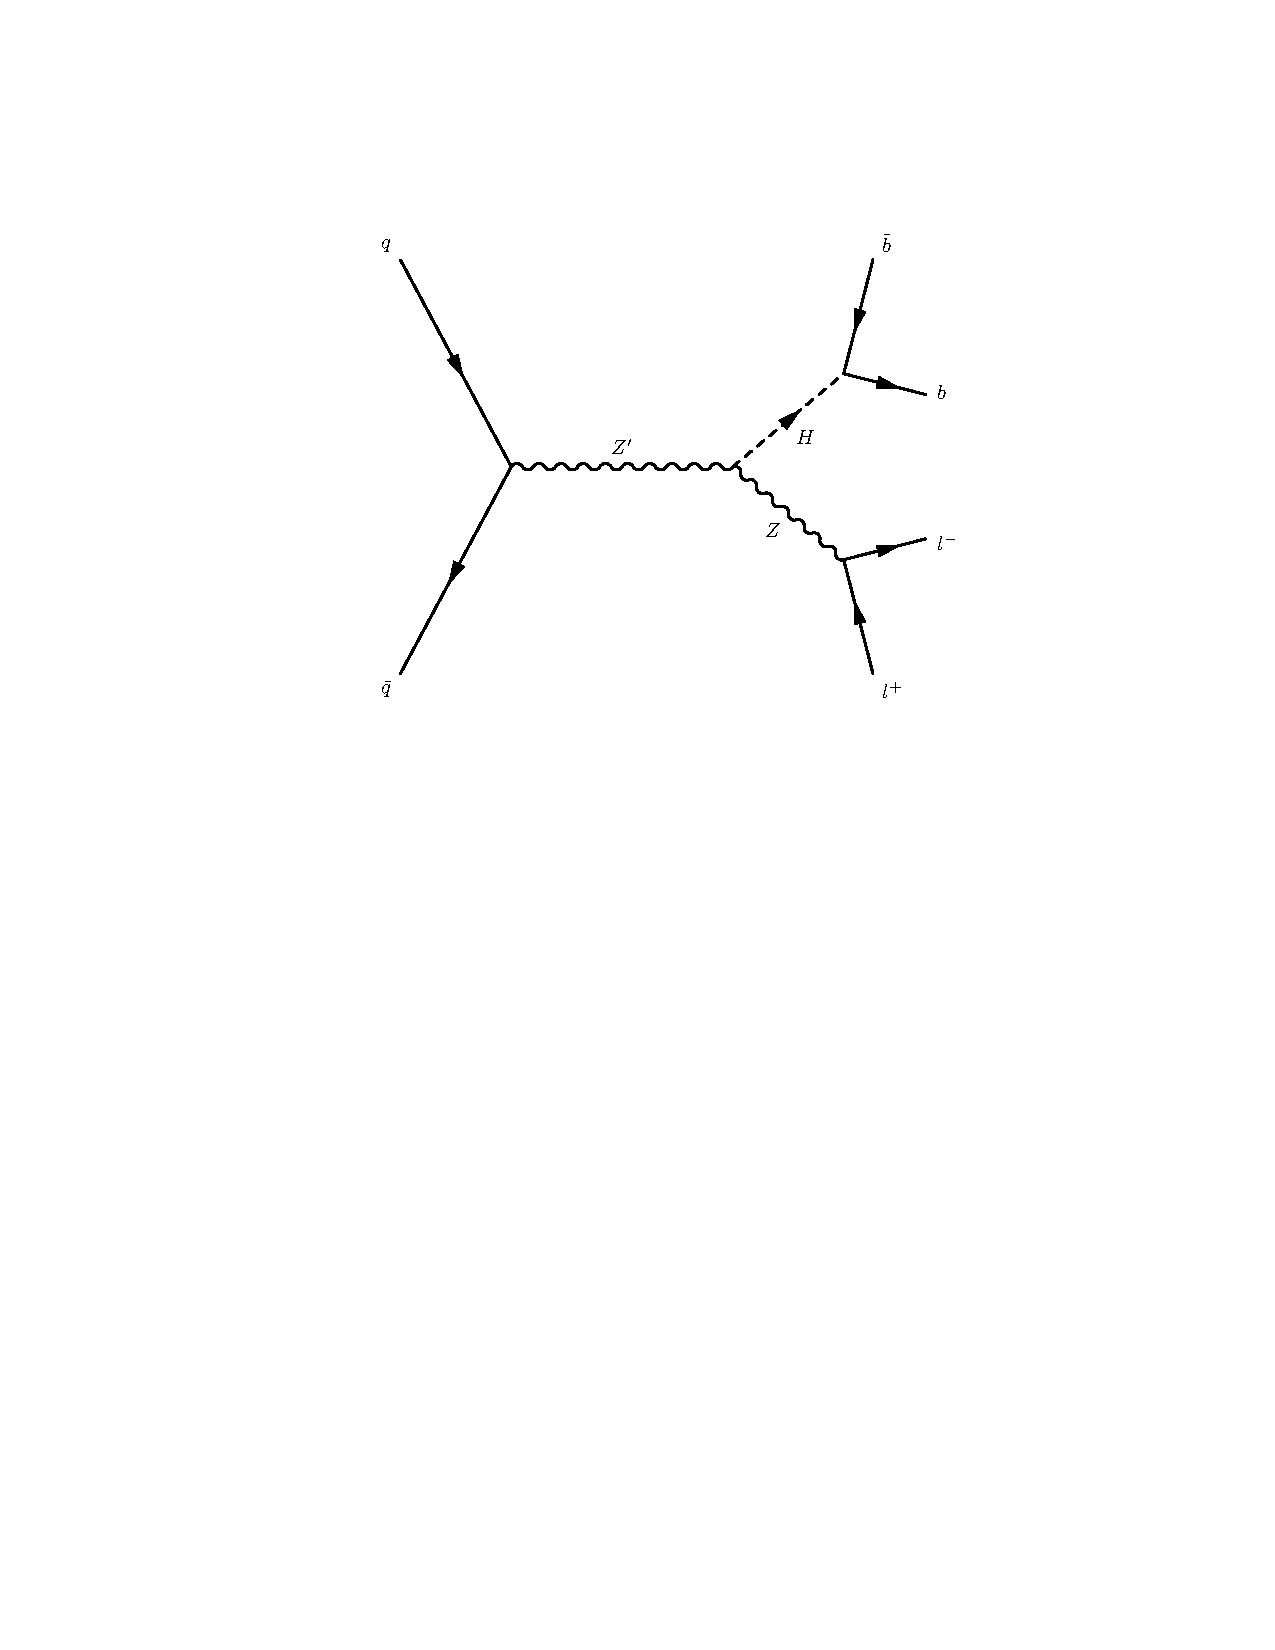
\includegraphics[width=1\textwidth,trim=0 400 0 100,clip=true]{Figures/feymann/qqZpZHllbb.pdf}
  \caption{Feymann diagram of the production of the heavy vector $Z'$, decaying into a $Z$ boson and a Higgs boson. The $Z$ boson further decays into two charged leptons, while the Higgs further decays into two $b$ quarks.}
  \label{fig:fey_signal}
\end{figure}

\section{Theoretical Motivations}

In the Standard Model (SM), the generation of masses for the weak gauge bosons ($W^\pm$ and $Z$) through electroweak symmetry breaking (EWSB) can be explained by the Higgs mechanism~\cite{PhysRevLett.13.508}. The mechanism was confirmed by the ATLAS and CMS experiments~\cite{Aad:2012tfa,Chatrchyan:2012xdj,Chatrchyan:2013lba} at the CERN 50 years after the theory has been proposed.

However, the discovered Higgs boson with mass of 125 GeV is much lighter than the Planck energy, which suggests that the SM may be incomplete. Various theories postulate the existence of new heavy resonances that couple to the SM bosons in an attempt to solve the hierarchy problem or naturalness problem. Some common models include the Little Higgs models~\cite{Han:2003wu,Perelstein:2005ka} and strongly coupled Composite Higgs~\cite{Contino:2011np,Marzocca:2012zn}. 

Various models can be generalized in the Heavy Vector Triplet (HVT) framework~\cite{Pappadopulo:2014qza}, which is a simplified approach based on a phenomenological Lagrangian. In the Simplified Model, only the relevant couplings and mass parameters are retained. The reason for this is that resonant searches are typically not sensitive to all the free parameters of the specific model, but only to those parameters that are related to the resonance mass and the interactions involved in its decay and production.

\subsection{Heavy Vector Triplet} \label{sec:hvtmodel}

Consider a heavy vector boson $V_\mu^a$, $a$ = 1,2,3, the simplified Lagrangian is described as
\begin{equation} \label{eq:simpleLag}
  \begin{aligned}
    \mathcal{L}_V = &-\frac{1}{4}D_{[\mu}V_{\nu]}^aD^{[\mu}V^{\nu]a}+\frac{m_V^2}{2}V_\mu^aV^{\mu a}\\
    &+ig_Vc_HV_\mu^aH^\dagger\tau^a\bar{D}^\mu H+\frac{g^2}{g_V}c_FV_\mu^a\sum\limits_{f}\bar{f}_L\gamma^\mu\tau^af_L\\
    &+\textup{quadrilinear terms}
  \end{aligned}
\end{equation}

The first term\footnote{The term \(D_{[\mu}V_{\nu]}^a = D_\mu V_\nu^a - D_\nu V_\mu^a\), where \(D_\mu V_\nu^a = \partial_\mu V_\nu^a + g\varepsilon^{abc}W_\mu^bV_\nu^c\).} in Eq.~\ref{eq:simpleLag} describes the interactions of $V$ with the SM weak bosons. The second term in the equation is the interactions of $V$ with itself, where the mass parameter $m_V$ does not coincide with the physical mass of the resonances. The third and fourth terms of the equation contains the interactions of $V$ with the Higgs current\footnote{The Higgs current term \(iH^\dagger\tau^a\bar{D}^\mu H = iH^\dagger\tau^aD^\mu H - iD^\mu H^\dagger\tau^aH\).} and with the SM left-handed fermionic currents\footnote{The fermionic currents \(\sum\bar{f}_L\gamma^\mu\tau^af_L\) involve the interactions of $V$ to leptons, light quarks and the third quarks family.}, respectively. The quadrilinear terms\footnote{The quadrilinear terms can be written as \[\frac{g_V}{2}c_{VVV}\varepsilon_{abc}V_\mu^aV_\nu^bD^{[\mu}V^{\nu]c} + g_V^2c_{VVHH}V_\mu^aV^{\nu a}H^\dagger H - \frac{g}{2}c_{VVW}\varepsilon_{abc}W^{\mu\nu a}V_\mu^bV_\nu^c.\]} do not contribute directly to $V$ decays and single production processes, therefore these terms can be disregarded.

In Eq.~\ref{eq:simpleLag}, besides the $SU$(2)$_L$ coupling constant $g$, another coupling constant $g_V$ is introduced to represent the strength of $V$ interactions. In addition, the term $c_H$ describes the $V$ interactions with the SM vector bosons and with the Higgs. Similarly, the term $c_F$ describes the $V$ interactions with fermions. They are expected to be of the order of unity in most models. 

\subsubsection*{Masses}

After the EWSB, only the photon stays massless due to the unbroken $U$(1)$_{EM}$, while the weak bosons acquire a mass and a mixing with heavy vector $V$. The mass matrix of the ($Z$, $V^0$) and the ($W^\pm$, $V^\pm$) are 
\begin{equation} \label{eq:matrixN}
  \mathcal{M}_N^2 =
  \begin{pmatrix}
    \hat{m}_Z^2 &
    c_H\xi\hat{m}_Z\hat{m}_V \\
    c_H\xi\hat{m}_Z\hat{m}_V &
    \hat{m}_V^2 \\
  \end{pmatrix}
\end{equation}
and
\begin{equation} \label{eq:matrixC}
  \mathcal{M}_C^2 =
  \begin{pmatrix}
    \hat{m}_W^2 &
    c_H\xi\hat{m}_W\hat{m}_V \\
    c_H\xi\hat{m}_W\hat{m}_V &
    \hat{m}_V^2 \\
  \end{pmatrix}
\end{equation}
respectively, where
\[\hat{m}_Z = \frac{e}{2\sin\theta_W\cos\theta_W}\hat{v}\]
\[\hat{m}_W = \cos\theta_W\hat{m}_Z\]
\[\hat{m}_V^2 = m_V^2 + g_V^2c_{VVHH}\hat{v}^2\]
\[\xi = \frac{g_V\hat{v}}{2\hat{m}_V}\]
Note that $e \approx \sqrt{4\pi/137}$, $\hat{v}$ is the Higgs field Vacuum Expectation Value, which has a value of 246 GeV, and $\theta_W$ is the weak mixing angle.

By taking the determinant of the mass matrices in Eq.~\ref{eq:matrixN} and Eq.~\ref{eq:matrixC}, the relation of the physical masses $M$ between charged and neutral heavy vectors are connected by $\theta_W$.
\begin{equation}
  m_W^2M_\pm^2 = \cos^2\theta_Wm_Z^2M_0^2
\end{equation}

In the experimental searches, the masses of new vectors should be at or above TeV scale, but the masses of SM bosons $m_{W,Z}$ should be preserved at about 100 GeV. A hierarchy in the mass spectrum is required to have
\begin{equation} \label{eq:massLimit}
  \frac{\hat{m}_{W,Z}}{\hat{m}_V} \sim \frac{m_{W,Z}}{M_{\pm,0}} \ll 1
\end{equation}

Under the limit in Eq.~\ref{eq:massLimit}, by expanding the determinant of the mass matrices in Eq.~\ref{eq:matrixN} and Eq.~\ref{eq:matrixC}, a simple approximate expressions for $m_W$ and $m_Z$ are given by
\[m_Z^2 \approx \hat{m}_Z^2(1-c_H^2\xi^2)\]
\[m_W^2 \approx \hat{m}_W^2(1-c_H^2\xi^2)\]
Since $\hat{m}_W = \cos\theta_W\hat{m}_Z$, the $W$-$Z$ mass ratio is given by 
\begin{equation} \label{eq:weakMass}
  \frac{m_W^2}{m_Z^2} \simeq \cos^2\theta_W
\end{equation}

Experimentally, the value of $\cos^2\theta_W$ is about 0.77. The charged and neutral $V$s are degenerated by
\begin{equation} \label{eq:hvtMass}
  M_\pm^2 = M_0^2 (1+\mathcal{O}(\%))
\end{equation}

It is clear that the mass splitting of charged and neutral states of $V$ is small enough to be ignored. This implies that the two states have comparable production rates.

\subsubsection*{Decay Widths}

Given that the mixing angles between weak bosons and $V$ are small due to the hierarchy in the mass spectrum, the couplings of the neutral and charged $V$ to left- and right-handed fermion chiralities can be written as
\begin{equation} \label{eq:LRcoupling}
  \begin{cases}
    g_L^N \simeq\frac{g^2}{g_V}\frac{c_F}{2}, \quad g_R^N \simeq 0 \\
    g_L^C \simeq\frac{g^2}{g_V}\frac{c_F}{\sqrt{2}}, \quad g_R^C = 0
  \end{cases}
\end{equation}
The ($g_{L,R}^{W,Z}$)$_{SM}$ in the Eq.~\ref{eq:LRcoupling} is the ordinary SM $W$ and $Z$ couplings with a normalization of $g_L^W = g/\sqrt{2}$. The $g$ is electroweak coupling which has a value of 0.65.

The decay width $\Gamma$ for fermionic channels can be written as
\begin{equation} \label{eq:fermionWidth}
  \Gamma_{V_\pm\rightarrow f\bar{f}'} \simeq 2\Gamma_{V_0\rightarrow f\bar{f}} \simeq N_c[f](\frac{g^2c_F}{g_V})^2\frac{M_V}{48\pi}
\end{equation}
where $N_c[f]$ is the number of colors (3 for di-quarks and 1 for di-leptons). The parameters $c_F={c_l,c_q,c_3}$ control the relative branching ratios (BR) to leptons, light quarks and the third family quarks.

The decay width for bosonic channels are
\begin{equation} \label{eq:bosonWidth}
  \Gamma_{V_0\rightarrow W_L^+W_L^-}\simeq\Gamma_{V_\pm\rightarrow W_L^\pm Z_L}\simeq\Gamma_{V_0\rightarrow Z_Lh}\simeq\Gamma_{V_\pm\rightarrow W_L^\pm h}\simeq\frac{g_V^2c_H^2M_V}{192\pi}[1+\mathcal{O}(\xi^2)]
\end{equation}
The channels that are not reported in the Eq.~\ref{eq:fermionWidth} and Eq.~\ref{eq:bosonWidth} are either forbidden or suppressed.

Since the $M_V$ is in the order of TeV scale, the $\xi$ should be very small. In this case, for a given resonance mass, the decay widths are fixed by the couplings $g^2c_F/g_V$ and $g_Vc_H$. The BRs and the production rate are controlled by the two parameters $g^2c_F/g_V$ and $g_Vc_H$.

\begin{figure}[t]
  \centering
  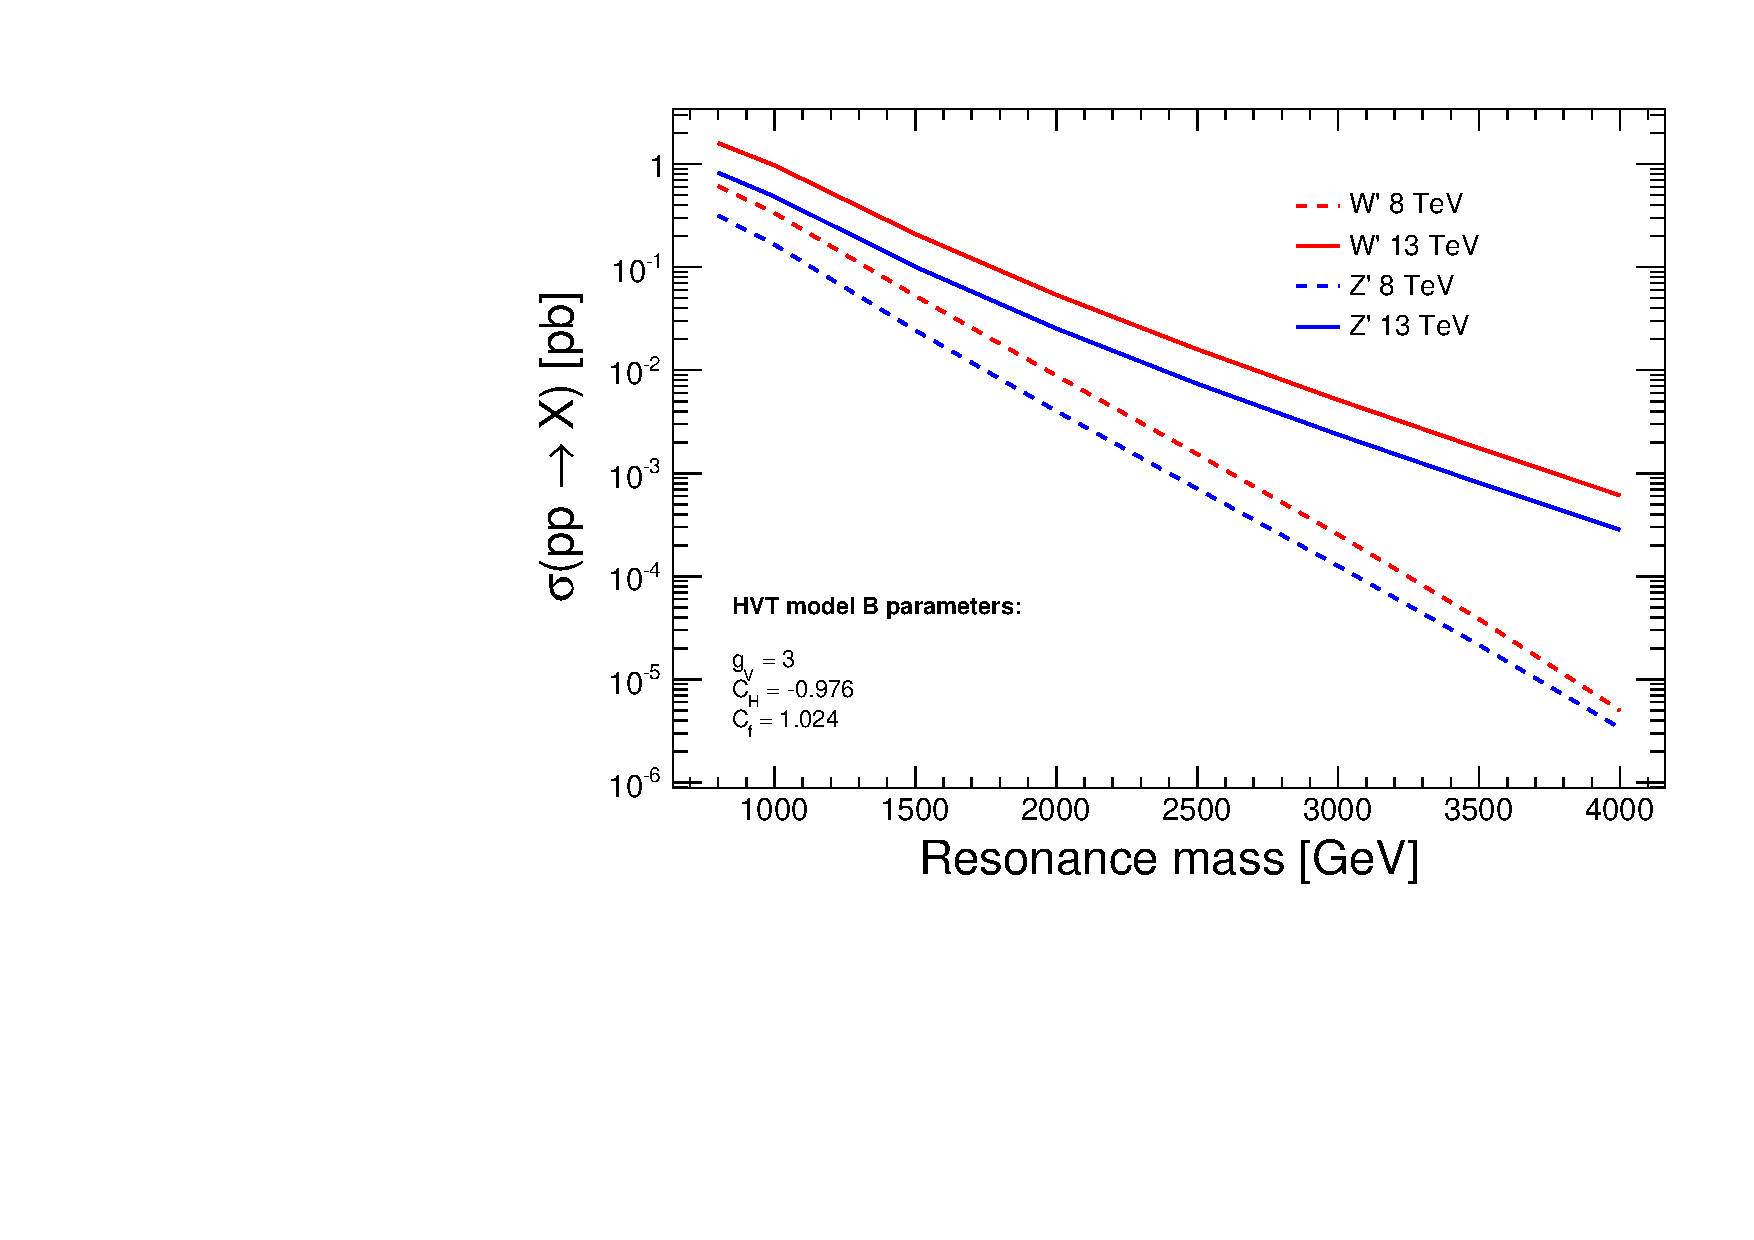
\includegraphics[width=0.55\textwidth]{Figures/hvt-xsec.pdf}
  \caption{Theoretical production cross section as a function of resonance mass for HVT Minimal Composite Higgs Model.}
  \label{fig:hvt_xsec}
\end{figure}

\subsection{Explicit Model} \label{sec:modelb}

It is now clear that the explicit model can be entirely described in terms of the two couplings $g^2c_F/g_V$ and $g_Vc_H$ and the mass $M_V$ with a good approximation~\cite{Pappadopulo:2014qza}.

Consider a strongly coupled scenario, so called Minimal Composite Higgs Model, where the Higgs doublet emerges from the spontaneous symmetry breaking of a global $SO$(5) symmetry to an $SO$(4) subgroup. In this scenario, the parameters $c_H$ and $c_F$ are fixed, \[c_H \sim -1, \quad c_F \sim 1\]

In addition, $g_V \gtrsim$ 3 is set to represent the strong coupling. In this case, the dominant BRs are bosonic decays due to $g_Vc_H \simeq -g_V$ in Eq.~\ref{eq:bosonWidth}, while the fermionic decays are extremely suppressed due to $g^2c_F/g_V \simeq g^2/g_V$ in Eq.~\ref{eq:fermionWidth}.

The results of this model is particularly interesting for the present search, since it predicts signal cross sections in the order of $fb$ for resonances up to 2$\sim$3 TeV (Figure~\ref{fig:hvt_xsec}), branching ratios to vector bosons close to the unity (Figure~\ref{fig:hvt_brs}), and thus being accessible at the LHC Run-II.

If the coupling is very large (for example $g_V$ = 8), the total width will be increased since the width of decays to dibosons grows with $g_V$ from Eq.~\ref{eq:bosonWidth}. But a very large coupling leads to an extremely broad resonance, which is not interesting to the experimental searches for a narrow resonance. Therefore, the $g_v$ has been constrained by $g_V \lesssim 4\pi$.

\begin{figure}[t]
  \centering
  \begin{tabular}{cc}
    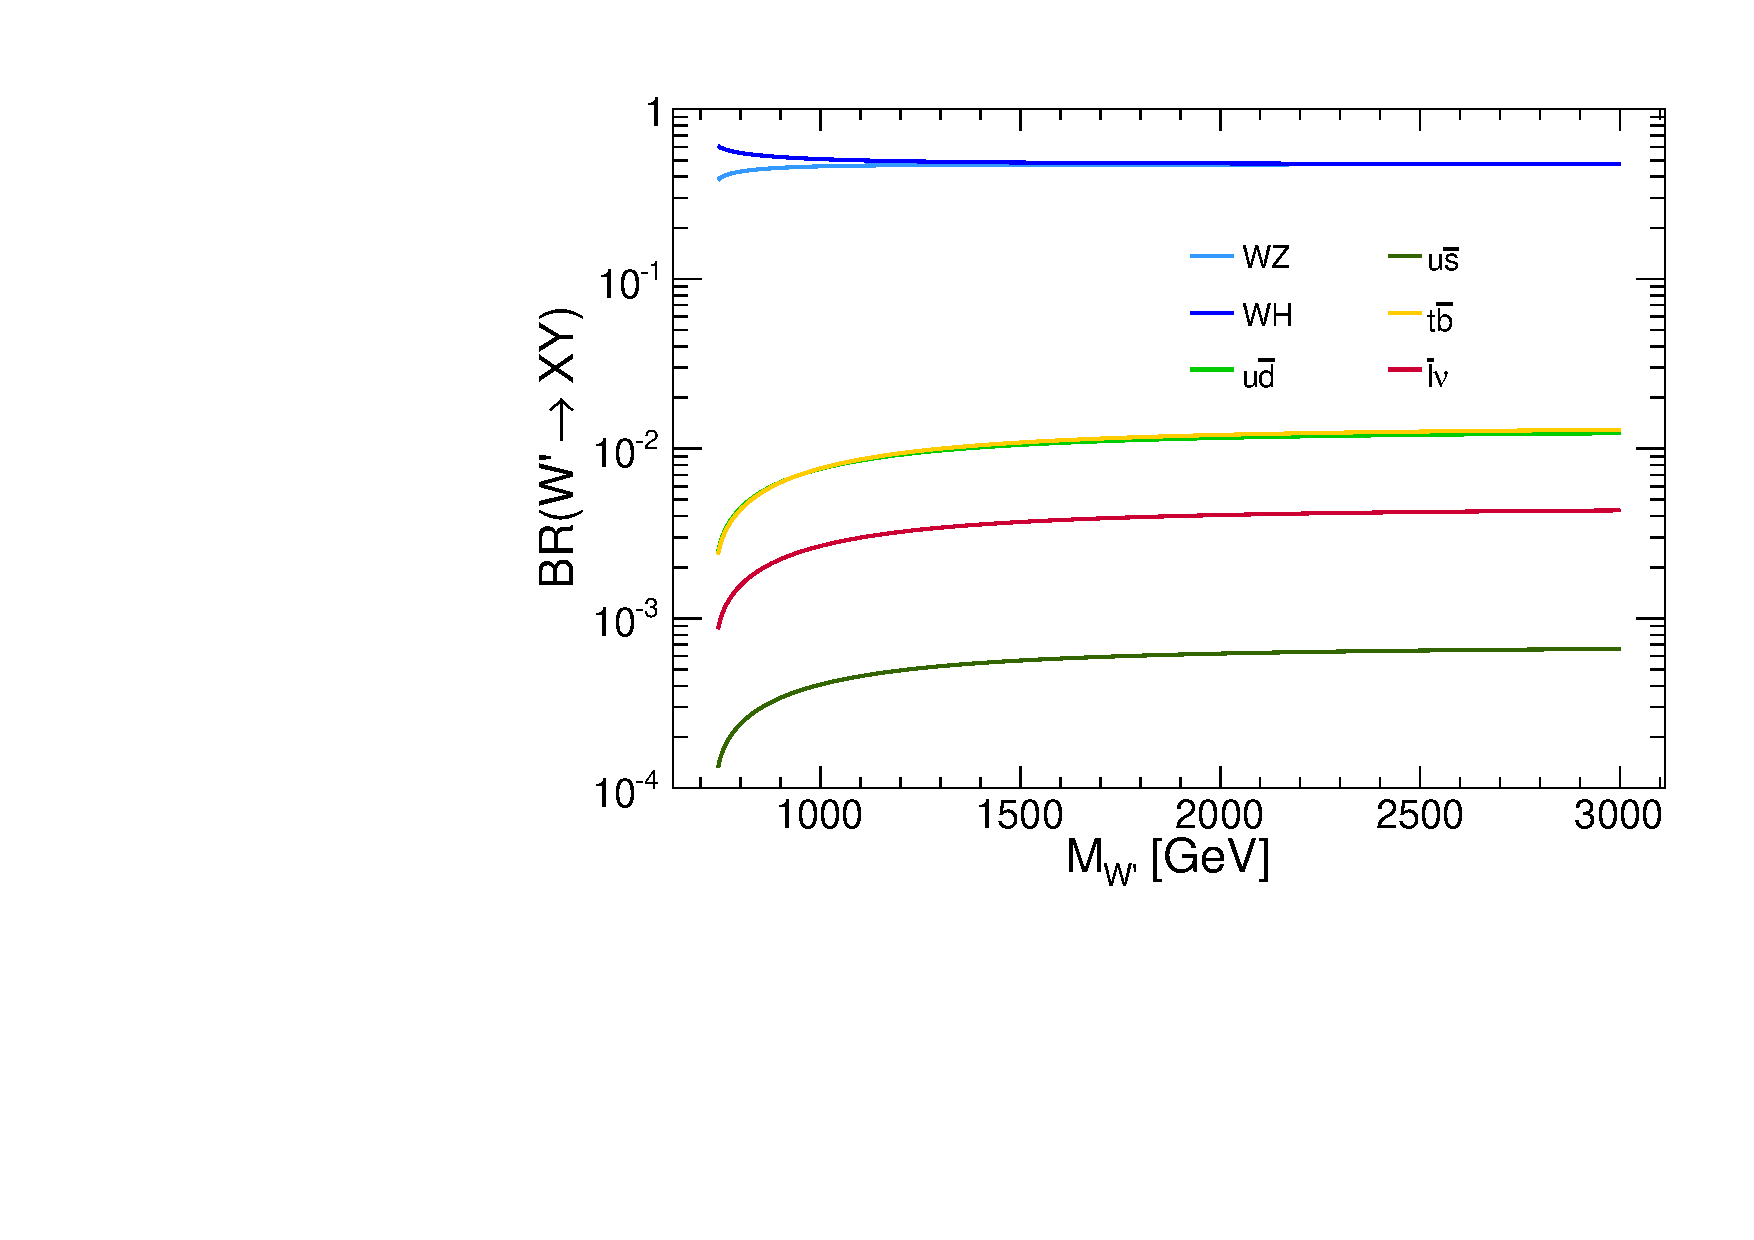
\includegraphics[width=0.5\textwidth]{Figures/hvt-wp-brs.pdf} &
    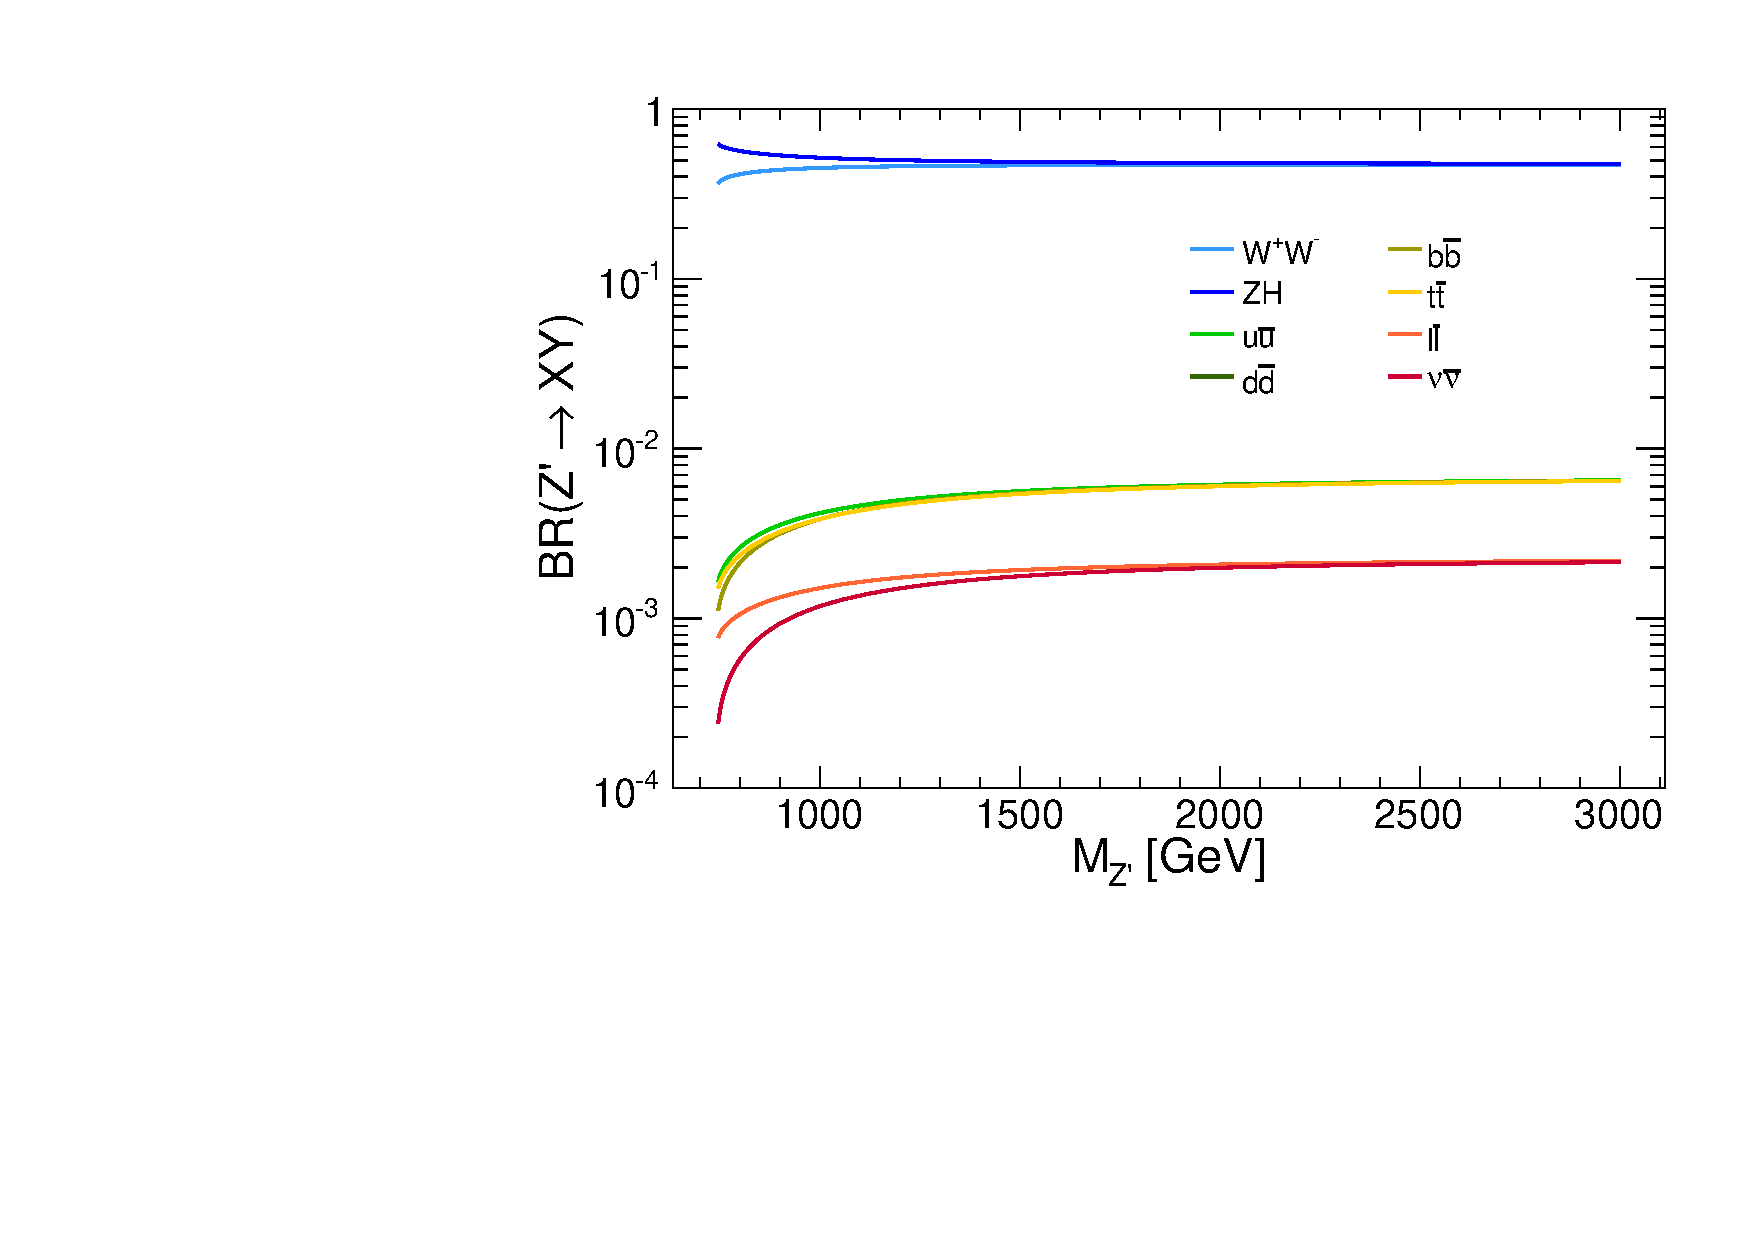
\includegraphics[width=0.5\textwidth]{Figures/hvt-zp-brs.pdf} \\
  \end{tabular}
  \caption{Branching ratios as a function of the resonance mass for a W' (left) and Z' (right) in the HVT Minimal Composite Higgs Model.}
  \label{fig:hvt_brs}
\end{figure}
